% Author: Izaak Neutelings (July 2018)
\documentclass[border=3pt,tikz]{standalone}
\usepackage{amsmath}
\usepackage{tikz}
\tikzset{>=latex} % for LaTeX arrow head
%\usepackage{xcolor}
%\colorlet{charge+}{blue!80!white}
\tikzstyle{charge0}=[top color=green!80!black!50,bottom color=green!80!black,shading angle=20]
\tikzstyle{charge+}=[top color=red!50,bottom color=red!70!black,shading angle=20]
\tikzstyle{charge-}=[top color=blue!50,bottom color=blue!80,shading angle=20]
%\tikzstyle{charge+}=[thin,ball color=blue!60,shading angle=-10]
%\tikzstyle{charge-}=[thin,ball color=red!85,shading angle=-10]
%\tikzstyle{charge0}=[thin,ball color=green!80!black!80,shading angle=-10]



\def\d{0.8}
\def\R{1.0}
\def\N{{1.04*(\R+\d)}}


\begin{document}
\Large

% ATOM MODEL
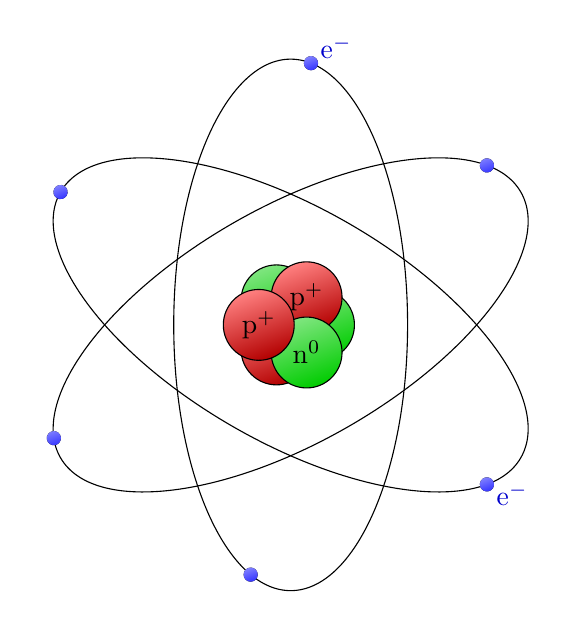
\begin{tikzpicture}[scale=0.45]
  
  \def\a{3.3}
  \def\b{7.5}
  \def\d{0.8}
  \def\D{0.9}
  \def\e{0.2} % electron radius
  
  
  \coordinate (O)  at (  0, 0);
  \coordinate (N1) at (  0:\d);
  \coordinate (N2) at (120:\d);
  \coordinate (N3) at (300:\D);
  \coordinate (P1) at (240:\d);
  \coordinate (P2) at ( 60:\D);
  \coordinate (P3) at (180:\D);
  
  % NUCLEUS
  \draw[charge0] (N1) circle (\R);
  \draw[charge0] (N2) circle (\R);
  \draw[charge+] (P1) circle (\R);
  \draw[charge+] (P2) circle (\R) node {$\text{p}^+$};
  \draw[charge0] (N3) circle (\R) node {$\text{n}^0$};
  \draw[charge+] (P3) circle (\R) node {$\text{p}^+$};
  
  % ELECTRONS
  \draw[rotate=  0] (0,0) ellipse ({\a} and {\b});
  \draw[rotate=120] (0,0) ellipse ({\a} and {\b});
  \draw[rotate=240] (0,0) ellipse ({\a} and {\b});
  \foreach \i/\ellipse/\theta [evaluate={\x=\a*cos(\theta-\ellipse); \y=\b*sin(\theta-\ellipse);}]
           in {1/0/80,2/0/250,3/120/50,4/120/200,5/240/150,6/240/-50}{
    \fill[charge-,rotate=\ellipse] (\x,\y) circle (\e) coordinate (E\i); %node[above right] {$\text{e}^-$};
  }
  
  \node[below=2,above right,blue!80!black] at (E1) {$\text{e}^-$};
  \node[below=-4,below right,blue!80!black] at (E6) {$\text{e}^-$};
  
\end{tikzpicture}


\end{document}